\documentclass[12pt,spanish]{report}
 \usepackage[T1]{fontenc}
 \usepackage{babel}
 \usepackage[round]{natbib}
 \usepackage{graphicx}
  \usepackage{hyperref}
 
 %%%%%%%%%%%%%%%%%%%%%%%%%%%
 
\def\apj{ApJ}%% Astrophysical Journal
 \def\apjl{ApJ}%% Astrophysical Journal, Letters
 %%%%%%%%%%%%%%%%%%%%%%%%%%%
 
 
 
 \author{Antonio Galv�n}
 \title{B�squeda de la contraparte electromagn�tica de ondas gravitacionales con el observatorio de rayos gamma HAWC}
 
\begin{document}
\maketitle
\tableofcontents

\chapter{Introducci�n}

Los destellos de Rayos Gamma (GRBs por su siglas en ingl�s)
\chapter{HAWC}

HAWC had a lot of bad lucky
\chapter{Una ventana hac�a la astrof�sica multimensajera: \newline WG170817/GRB170817A}

%El 17 de Agosto del 2017 el monitor de destellos de rayos gamma (GBM)\footnote{Por sus siglas en  ingl�s;  Gamma-Ray Burst Monitor} a bordo del sat�lite espacial FERMI  dispar� la alerta a las 12:41:06.47 UT \citep{2017GCN.21520....1V} de la detecci�n del GRB170817A la cual fue coincidente espacial y temporalmente (con un retraso de $\sim$2 s) con la detecci�n de ondas gravitacionales por parte de los interfer�metros LIGO y Virgo \citep{GCNGW...LW,GCNGW...LW2}. El hecho de que estas dos alarmas coincidieran significar�a la primera detecci�n de una kilonova, la contraparte electromagn�tica de ondas gravitacionales. A partir de este momento se inicio una campa�a intensiva de telescopios en distintas longitudes de onda \citep{2017ApJ...848L..12A}. La primer detecci�n en �ptico por telescopios terrestres fue realizada por el observatorio  LBT\footnote{Por sus siglas en  ingl�s; Large Binocular Telescope Observatory} \citep{2017GCN.21520....2V}. Nueve d�as despu�s se detecta emisi�n de rayos X \textbf{[??]} en la posici�n de la onda gravitacional 

El 17 de Agosto de 2017 a las 12:41:06.47 UT el monitor de rayos gamma (GBM)\footnote{Por sus siglas en  ingl�s;  Gamma-Ray Burst Monitor} a bordo del sat�lite espacial FERMI disparar�a la alerta del Destello de Rayos Gamma  (de ahora en adelante GRB) corto GRB170817A  \citep{2017GCN.21520....1V}. Apuntaba a ser otro de los $\sim$2 GRBs detectados cada semana, generando la GCN correspondiente 14 segundos despu�s del destello. Seis minutos despu�s, en la tierra, el interferometro LIGO \footnote{(Por sus siglas en ingl�s, Laser Interferometer Gravitational-wave Observatory)} en Hanford, aparec�a un candidato a onda gravitacional en \textit{latencia baja}. Este candidato tomo relevancia debido a que era consistente con un evento coalescente de dos estrellas de neutrones y coincidente con una diferencia de $\sim$ 2 segundos del GRB170817A \citep{GCNGW...LW,GCNGW...LW2}.

 En la figura \ref{Fig1} se muestra la fracci�n del cielo en los cuales Fermi-GBM (combinando con datos de INTEGRAL para poder disminuir la incertidumbre) y LIGO (Considerando datos de Hanford y Livingston as� como de VIRGO) detectaron la onda gravitacional. Finalmente la oportuna detecci�n en la banda del �ptico por el LBT\footnote{Por sus siglas en  ingl�s; Large Binocular Telescope Observatory} \citep{2017GCN.21520....2V} permite tener certeza de la posici�n del GRB as� como de la galaxia anfitriona; NGC 4993 \citep{2017Sci...358.1556C}, la cual se encuentra a una distancia de 40 Mpc de la Tierra. Sin lugar a dudas este evento ha sido hasta el momento uno de los m�s cercanos registrados hasta la fecha y destinado a marcar un parte aguas dentro de la astrof�sica.
 
 \begin{figure}
  \centering
    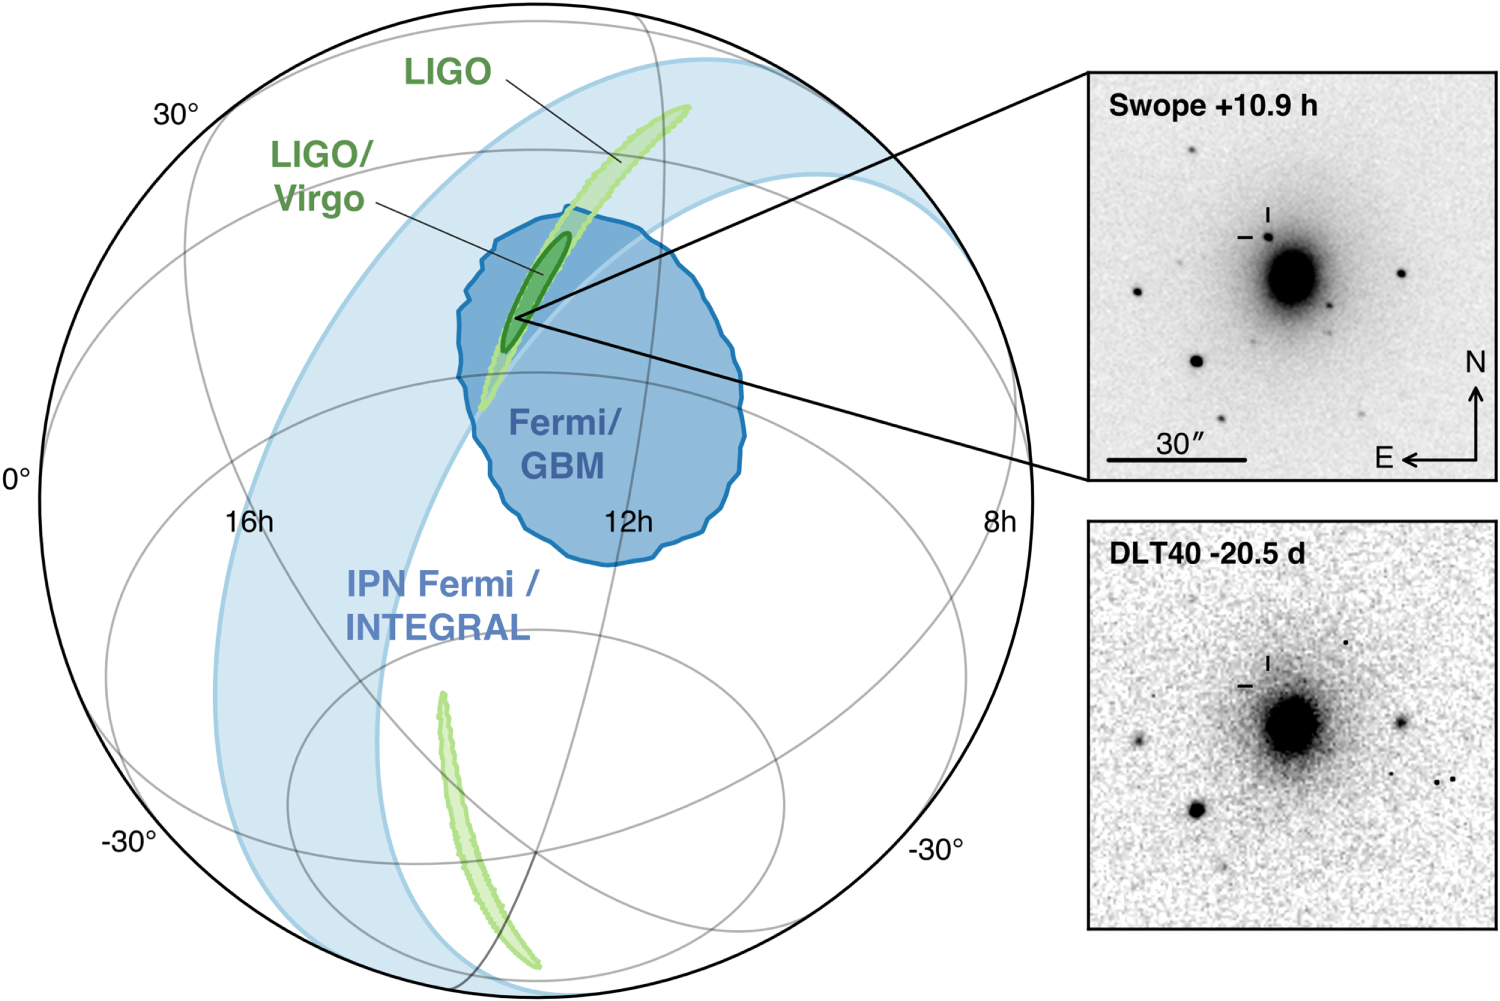
\includegraphics[width=0.9\textwidth]{./Figures/apjlaa91c9f1_hr.jpg}
      \caption{A picture of the GW. Imagen tomada de \citep{2017ApJ...848L..12A} \label{Fig1}}
\end{figure}

\section{Campa�as de observaci�n}
Las observaciones 24 hrs. post merger fue de gran importancia, ya sea, tratando de poder determinar una posible galaxia anfitriona as� como de poder descartar si el afterglow detectado podr�a estar correlacionado a otro fen�meno. As� como de la eventual detecci�n de rayos-X como la emisi�n en radio. En la figura \ref{Fig2} se muestra una linea del tiempo de las observaciones a partir de la detecci�n de la onda gravitacional.

\subsection{Detecci�n de ondas gravitacionales}

\begin{figure}
  \centering
    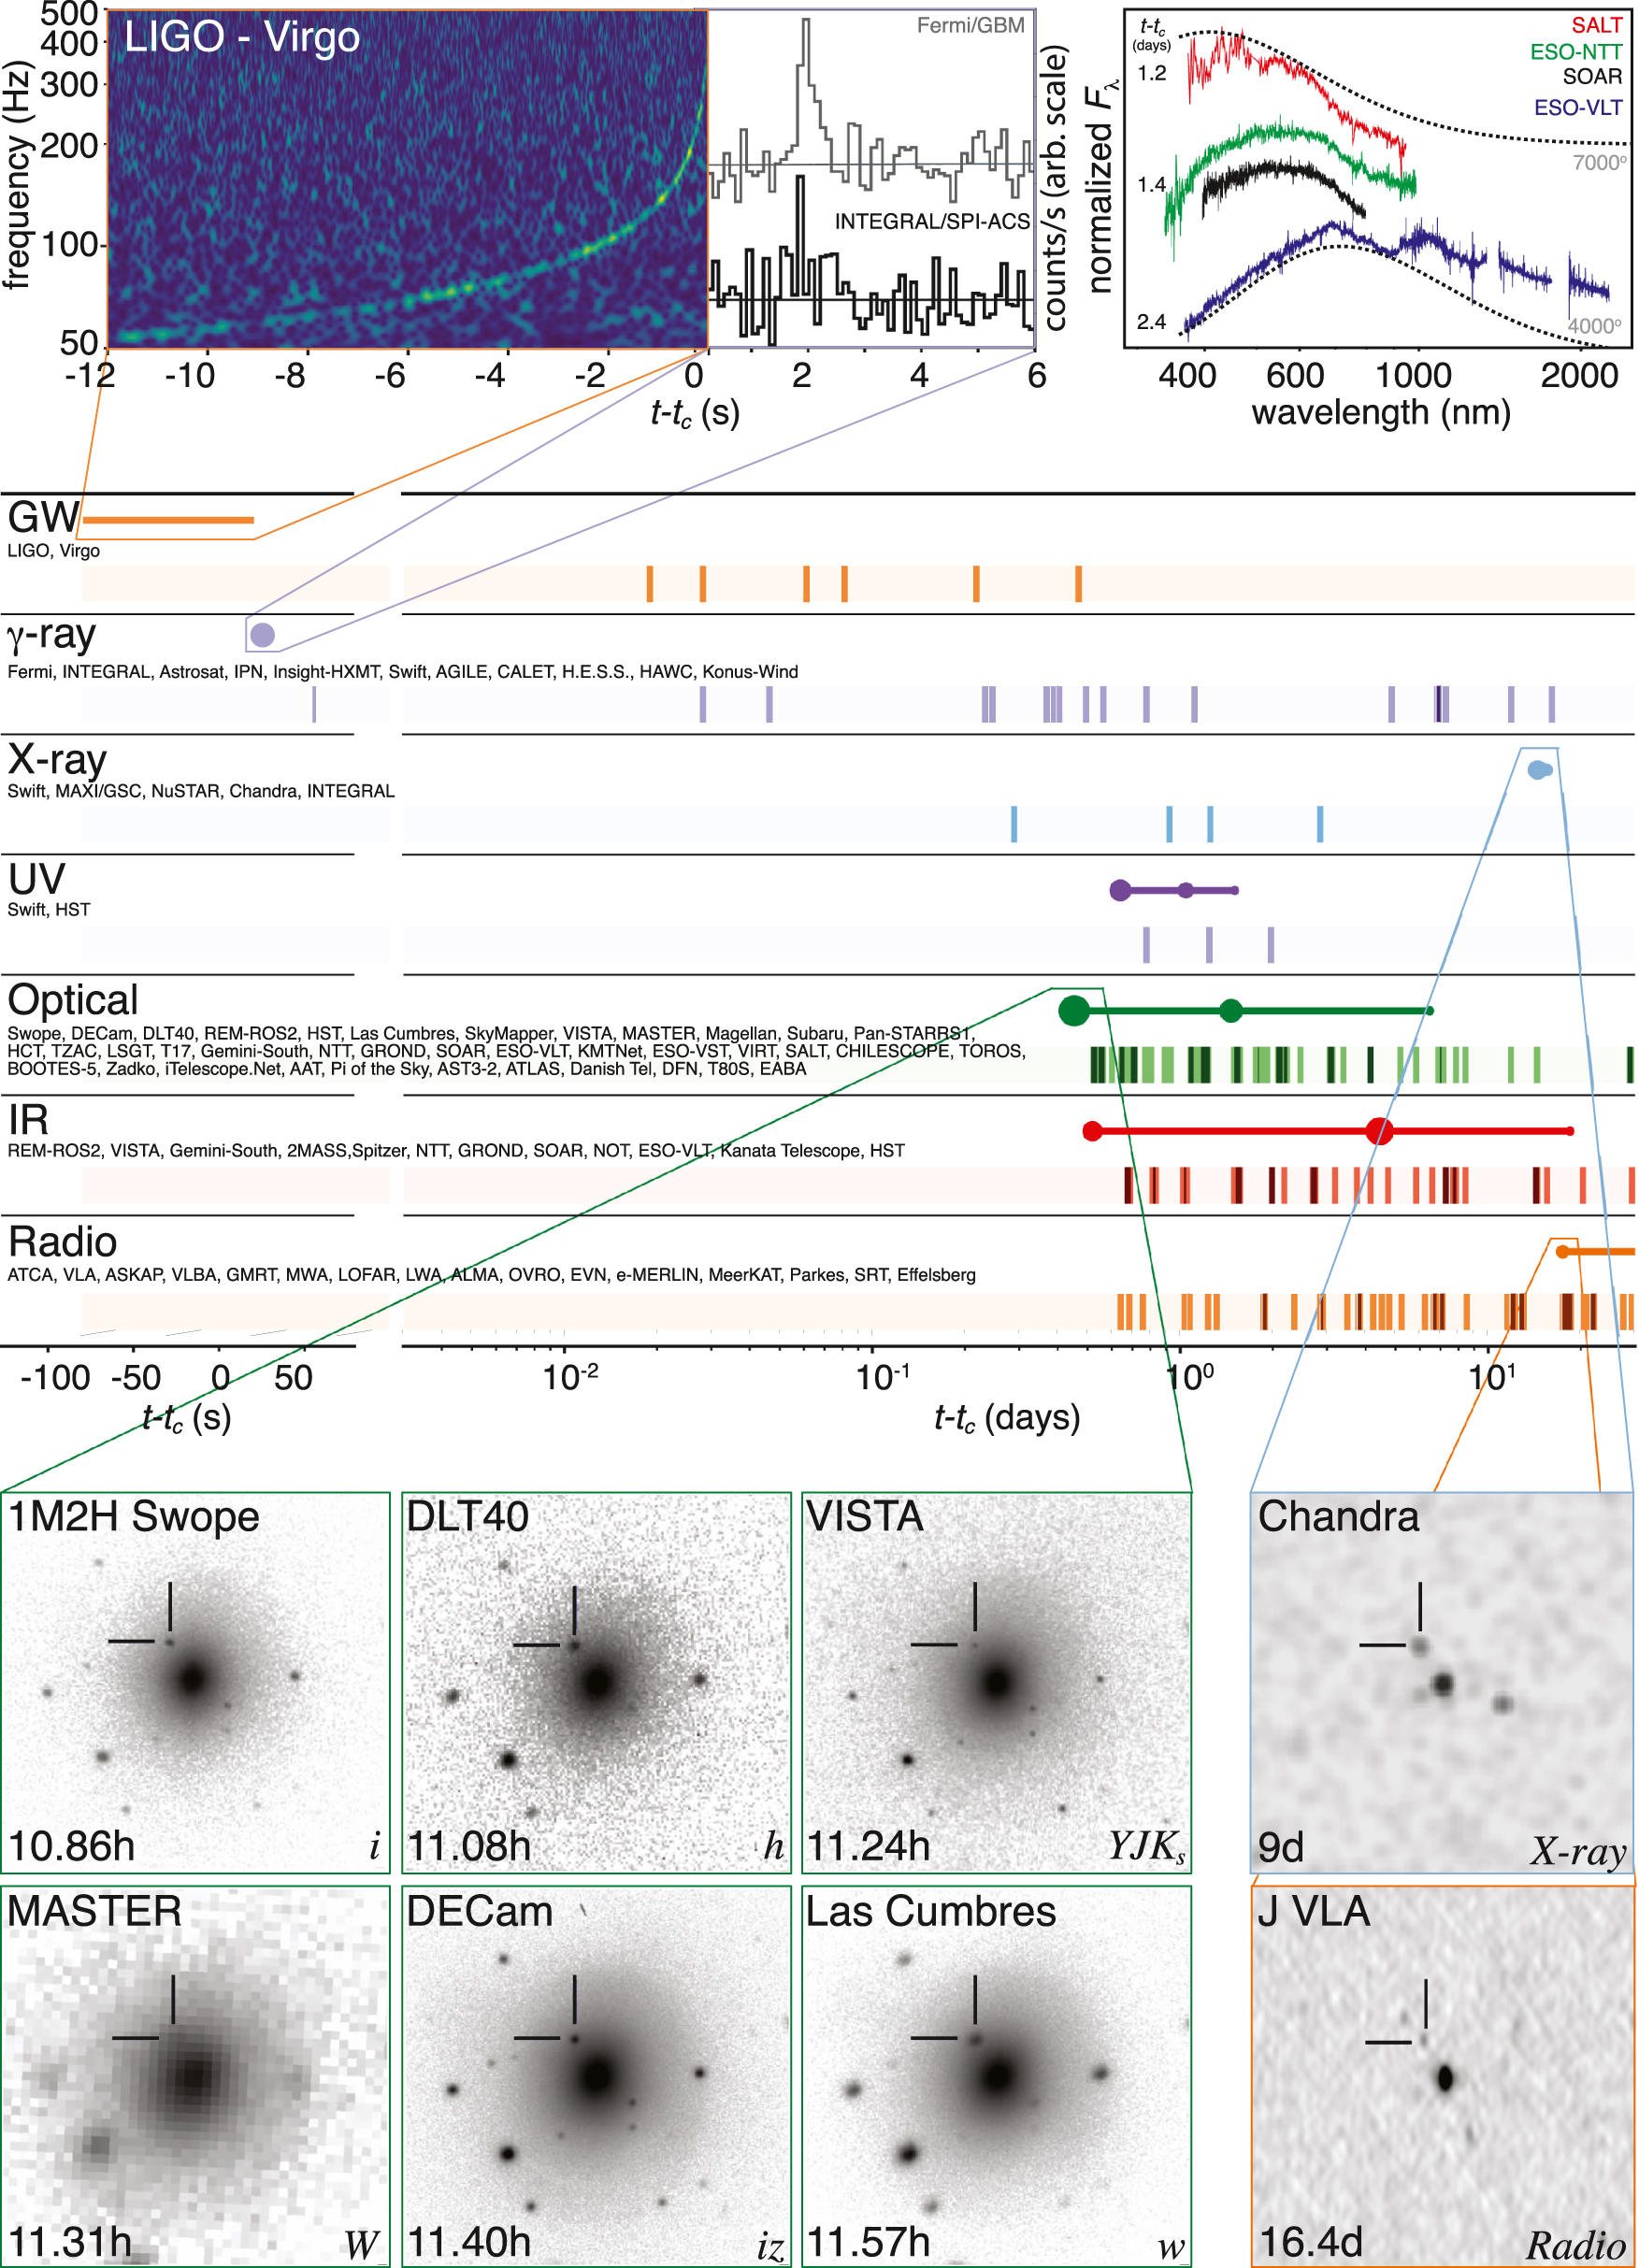
\includegraphics[width=0.9\textwidth]{./Figures/apjlaa91c9f2_hr.jpg}
      \caption{A picture of the GW. Imagen tomada de \citep{2017ApJ...848L..12A} \label{Fig2}}
\end{figure}



\chapter{Constrains using HAWC on GRB170817A}

Desafortunadamente, el evento de la onda gravitacional GW170817 ocurri� fuera del campo de visi�n de HAWC. Sin embargo, 8 hrs depu�s el tr�nsito logra entrar en el campo de visi�n del observatorio colocando un upper limit a XX \citep{2017ApJ...848L..12A}. Debido a la naturaleza que present� el afterglow de este GRB, en donde, apareci� la emisi�n de rayos X a 9 d�as \textbf{[??]} y de radio a 16 d�as \textbf{[??]} despu�s del destello respectivamente, alcanzando un flujo m�ximo a los \textcolor{red}{120 d�as} \textbf{[??]} se realiza un monitoreo a ciegas buscando  emisi�n en TeV's detectable por HAWC.


\section{Mapas del cielo de d�as siderales}

HAWC presenta su �ptima sensibilidad para fuentes que se encuentran dentro de las declinaciones -26$\degree$ y +64$\degree$, tal y como se muestra la regi�n sombreada en la figura \ref{fig:FOV-HAWC}. De esta manera definimos a un transito como la visibilidad de una fuente por HAWC la cual se encuentra con un �ngulo cenital $\theta$ < 45$\degree$. Un estudio m�s detallado presentado en \citep{2017ApJ...841..100A} muestra que la mayor cantidad de emisi�n de fuentes c�mo lo son la nebulosa del Cangrejo, y los Markarian 421 y 501 deber�an de detectarse dentro de las primeras 4 hrs del transito sobre HAWC. As� mismo los mapas inician a la media noche sideral de HAWC. Los mapas son dividos en mapas de 12 horas siderias, de tal forma que se genera una subclaficiaci�n, aquellas fuentes las cuales tienen una ascensi�n recta < 3 hrs �  > 21 hrs � bien, el complemento.

\begin{figure}[ht!]
  \centering{
  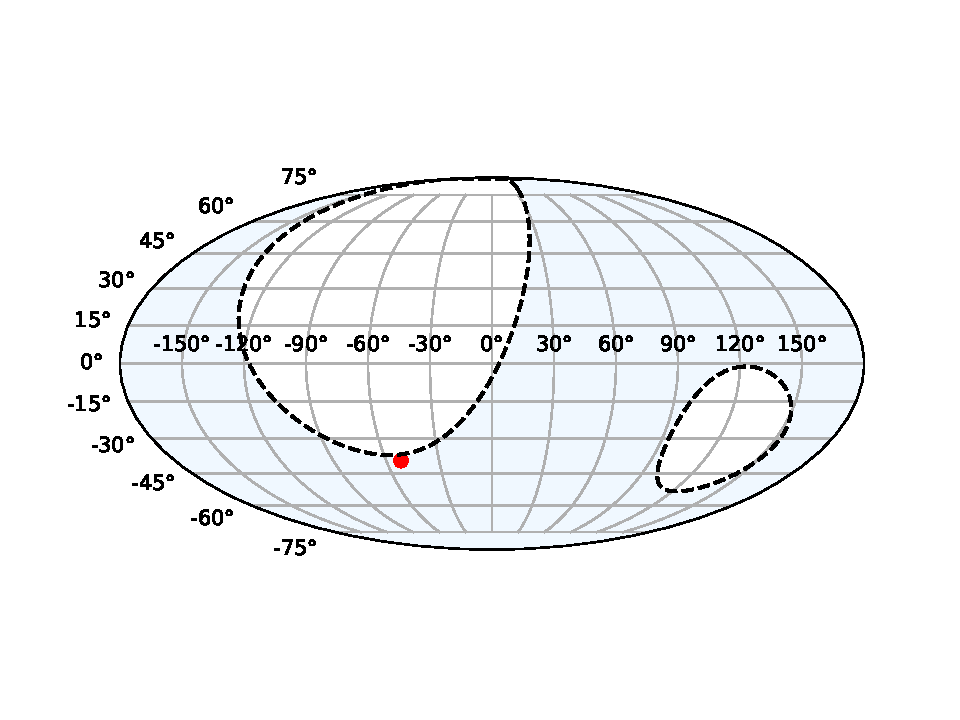
\includegraphics[width=1.0\linewidth]{Figures/HAWC_GW.pdf}}
  \caption{Campo de visi�n de HAWC}
  \label{fig:FOV-HAWC}
\end{figure}

Cada mapa sideral est� dividido en 9 bines en funci�n de la multiplicidad del primario \citep{2017ApJ...843...39A} y cada bin est� constituido por un mapa utilizando una malla de pixeles mediante HEALPix \citep{2005ApJ...622..759G}



\section{B�squeda tard�a en TeVs}
Considerando bines temporales de...
\chapter{Conclusiones}

Pues nada, resulta que...


\lipsum


\lipsum


\bibliographystyle{plainnat}
\bibliography{Bibliografia/bibliografia.bib} 



\end{document}

